\section{Evaluation}
\label{sec:evaluation}

Having proposed our enclave construction framework, we now evaluate it with respect to practicality, performance, and security.

\subsection{Performance}
\label{sec:performance}

\begin{itemize}
    \item Throughput. How much data can we shove through the VSOCK interface?
    \item Latency. What's the additional latency (if any) of talking to an application through the VSOCK interface compared to directly?
\end{itemize}

\subsubsection{Attestation Documents}
\label{sec:attestation-performance}

The fetching of attestation documents is a critical part of our framework's overall performance.  We wrote a stress test tool that requests as many attestation documents as it can over sixty seconds.  The tool is essentially a minimal enclave application that does nothing beyond requesting attestation documents.  For each attestation document, we asked the hypervisor to include an incrementing nonce, to avoid any speedups by caching.  We were able to receive approximately 900 documents per second, with each request taking a median of one millisecond ($s = 0.3\,\text{ms}$) to fetch the attestation document.\footnote{We performed our measurements on a c5.xlarge EC2 instance which comes with four CPUs and eight GiB of memory.}

Faster than Intel's attestation service~\cite{Chen2019a}?

\subsubsection{End-to-end Performance}
\label{sec:end-to-end}

Next, we set out to measure the networking throughput of the critical path, as illustrated in Figure~\ref{fig:stress-test}.  In particular, we test latency and throughput of our TCP proxy, the VSOCK interface between EC2 and enclave, and a minimal enclave application.  To rule out unnecessary computation in the enclave application, we implemented a simple service whose only job it is to respond with the string ``hello world'' when clients request the path /hello-world.  To simulate clients, we use the HTTP load test tool Baton~\cite{baton}, which sends concurrent HTTP requests to the application.  We run Baton on the parent EC2 instance and make it send requests to the TCP proxy.  Note that this test setup constitutes a \emph{lower bound} of the performance that is achievable.  Real-world applications will be slower because clients send their request over the Internet (which adds latency) and the enclave application is likely to be more complex (which adds latency).

\begin{figure}[t]
    \centering
    \begin{tikzpicture}[node distance=20pt]
  \node [draw,
         label={[anchor=north]above:EC2 host},
         minimum height=40pt,
         align=center,
         minimum width=110pt] (ec2) {};

  \node [draw,
         label={[anchor=north]above:Enclave},
         right=0pt of ec2,
         fill=black!10,
         minimum height=40pt,
         minimum width=120pt] (enclave) {};

  \node [draw,
         align=center,
         yshift=-5pt,
         left=10pt of ec2.east] (proxy) {Proxy};

  \node [draw,
         align=center,
         left=of proxy] (baton) {Baton};

  \node [draw,
         align=center,
         fill=white,
         yshift=-5pt,
         right=10pt of enclave.west] (nitriding) {Nitriding};

  \node [draw,
         align=center,
         fill=white,
         right=of nitriding] (app) {Web srv};

  \node [xshift=15pt,
         yshift=-5pt,
         align=center] at (enclave.north west)
    {\footnotesize \color{gray} VSOCK};

  % Baton talking to the Web service.
  \draw[-latex] ([yshift=5pt]baton.east) -- ([yshift=5pt]proxy.west);
  \draw[-latex] (baton.east) -- (proxy.west);
  \draw[-latex] ([yshift=-5pt]baton.east) -- ([yshift=-5pt]proxy.west);

  \draw[-latex] ([yshift=5pt]proxy.east) -- ([yshift=5pt]nitriding.west);
  \draw[-latex] (proxy.east) -- (nitriding.west);
  \draw[-latex] ([yshift=-5pt]proxy.east) -- ([yshift=-5pt]nitriding.west);

  \draw[-latex] ([yshift=5pt]nitriding.east) -- ([yshift=5pt]app.west);
  \draw[-latex] (nitriding.east) -- (app.west);
  \draw[-latex] ([yshift=-5pt]nitriding.east) -- ([yshift=-5pt]app.west);

\end{tikzpicture}

    \label{fig:stress-test}
    \caption{Our stress test tool tests the performance of our critical path, consisting of the TCP proxy, the VSOCK interface, and Go's HTTP stack in the enclave application.}
\end{figure}

\begin{figure}[t]
    \centering
    \begin{tabular}{l r r r}
    \toprule
    Setup & Reqs/sec & Mean lat. & Max lat. \\
    \midrule
    Full & ~7,500 & 12.7 & 56.0 \\
    No proxy & 14,100 & 6.5 & 52.0 \\
    Direct & ~27,900 & 3.2 & 50.0 \\
    \bottomrule
    \end{tabular}
    \caption{Using 100 concurrent requests and 100,000 requests in total.}
    \label{tab:my_label}
\end{figure}


\begin{figure}[t]
    \centering
    % Created by tikzDevice version 0.12.3.1 on 2023-01-22 18:15:41
% !TEX encoding = UTF-8 Unicode
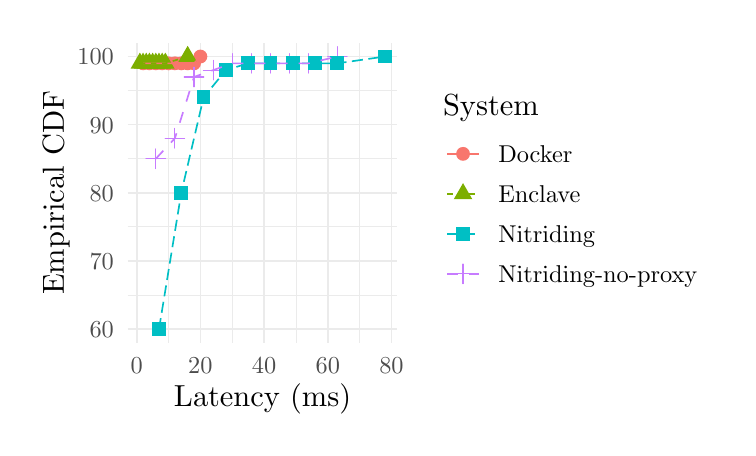
\begin{tikzpicture}[x=1pt,y=1pt]
\definecolor{fillColor}{RGB}{255,255,255}
\path[use as bounding box,fill=fillColor,fill opacity=0.00] (0,0) rectangle (252.94,144.54);
\begin{scope}
\path[clip] ( 36.11, 30.69) rectangle (133.59,139.04);
\definecolor{drawColor}{gray}{0.92}

\path[draw=drawColor,line width= 0.3pt,line join=round] ( 36.11, 47.92) --
	(133.59, 47.92);

\path[draw=drawColor,line width= 0.3pt,line join=round] ( 36.11, 72.55) --
	(133.59, 72.55);

\path[draw=drawColor,line width= 0.3pt,line join=round] ( 36.11, 97.18) --
	(133.59, 97.18);

\path[draw=drawColor,line width= 0.3pt,line join=round] ( 36.11,121.80) --
	(133.59,121.80);

\path[draw=drawColor,line width= 0.3pt,line join=round] ( 50.90, 30.69) --
	( 50.90,139.04);

\path[draw=drawColor,line width= 0.3pt,line join=round] ( 73.92, 30.69) --
	( 73.92,139.04);

\path[draw=drawColor,line width= 0.3pt,line join=round] ( 96.94, 30.69) --
	( 96.94,139.04);

\path[draw=drawColor,line width= 0.3pt,line join=round] (119.95, 30.69) --
	(119.95,139.04);

\path[draw=drawColor,line width= 0.6pt,line join=round] ( 36.11, 35.61) --
	(133.59, 35.61);

\path[draw=drawColor,line width= 0.6pt,line join=round] ( 36.11, 60.24) --
	(133.59, 60.24);

\path[draw=drawColor,line width= 0.6pt,line join=round] ( 36.11, 84.86) --
	(133.59, 84.86);

\path[draw=drawColor,line width= 0.6pt,line join=round] ( 36.11,109.49) --
	(133.59,109.49);

\path[draw=drawColor,line width= 0.6pt,line join=round] ( 36.11,134.11) --
	(133.59,134.11);

\path[draw=drawColor,line width= 0.6pt,line join=round] ( 39.39, 30.69) --
	( 39.39,139.04);

\path[draw=drawColor,line width= 0.6pt,line join=round] ( 62.41, 30.69) --
	( 62.41,139.04);

\path[draw=drawColor,line width= 0.6pt,line join=round] ( 85.43, 30.69) --
	( 85.43,139.04);

\path[draw=drawColor,line width= 0.6pt,line join=round] (108.45, 30.69) --
	(108.45,139.04);

\path[draw=drawColor,line width= 0.6pt,line join=round] (131.46, 30.69) --
	(131.46,139.04);
\definecolor{fillColor}{RGB}{248,118,109}

\path[fill=fillColor] ( 41.69,131.65) circle (  2.50);

\path[fill=fillColor] ( 43.99,131.65) circle (  2.50);

\path[fill=fillColor] ( 46.30,131.65) circle (  2.50);

\path[fill=fillColor] ( 48.60,131.65) circle (  2.50);

\path[fill=fillColor] ( 50.90,131.65) circle (  2.50);

\path[fill=fillColor] ( 53.20,131.65) circle (  2.50);

\path[fill=fillColor] ( 55.50,131.65) circle (  2.50);

\path[fill=fillColor] ( 57.81,131.65) circle (  2.50);

\path[fill=fillColor] ( 60.11,131.65) circle (  2.50);

\path[fill=fillColor] ( 62.41,134.11) circle (  2.50);
\definecolor{fillColor}{RGB}{124,174,0}

\path[fill=fillColor] ( 40.54,135.54) --
	( 43.91,129.71) --
	( 37.18,129.71) --
	cycle;

\path[fill=fillColor] ( 41.69,135.54) --
	( 45.06,129.71) --
	( 38.33,129.71) --
	cycle;

\path[fill=fillColor] ( 42.84,135.54) --
	( 46.21,129.71) --
	( 39.48,129.71) --
	cycle;

\path[fill=fillColor] ( 43.99,135.54) --
	( 47.36,129.71) --
	( 40.63,129.71) --
	cycle;

\path[fill=fillColor] ( 45.15,135.54) --
	( 48.51,129.71) --
	( 41.78,129.71) --
	cycle;

\path[fill=fillColor] ( 46.30,135.54) --
	( 49.66,129.71) --
	( 42.93,129.71) --
	cycle;

\path[fill=fillColor] ( 47.45,135.54) --
	( 50.81,129.71) --
	( 44.08,129.71) --
	cycle;

\path[fill=fillColor] ( 48.60,135.54) --
	( 51.96,129.71) --
	( 45.23,129.71) --
	cycle;

\path[fill=fillColor] ( 49.75,135.54) --
	( 53.11,129.71) --
	( 46.39,129.71) --
	cycle;

\path[fill=fillColor] ( 57.81,138.00) --
	( 61.17,132.17) --
	( 54.44,132.17) --
	cycle;
\definecolor{drawColor}{RGB}{199,124,255}

\path[draw=drawColor,line width= 0.4pt,line join=round,line cap=round] ( 42.76, 97.18) -- ( 49.83, 97.18);

\path[draw=drawColor,line width= 0.4pt,line join=round,line cap=round] ( 46.30, 93.64) -- ( 46.30,100.71);

\path[draw=drawColor,line width= 0.4pt,line join=round,line cap=round] ( 49.67,104.56) -- ( 56.73,104.56);

\path[draw=drawColor,line width= 0.4pt,line join=round,line cap=round] ( 53.20,101.03) -- ( 53.20,108.10);

\path[draw=drawColor,line width= 0.4pt,line join=round,line cap=round] ( 56.58,126.73) -- ( 63.64,126.73);

\path[draw=drawColor,line width= 0.4pt,line join=round,line cap=round] ( 60.11,123.19) -- ( 60.11,130.26);

\path[draw=drawColor,line width= 0.4pt,line join=round,line cap=round] ( 63.48,129.19) -- ( 70.55,129.19);

\path[draw=drawColor,line width= 0.4pt,line join=round,line cap=round] ( 67.01,125.66) -- ( 67.01,132.72);

\path[draw=drawColor,line width= 0.4pt,line join=round,line cap=round] ( 70.39,131.65) -- ( 77.45,131.65);

\path[draw=drawColor,line width= 0.4pt,line join=round,line cap=round] ( 73.92,128.12) -- ( 73.92,135.18);

\path[draw=drawColor,line width= 0.4pt,line join=round,line cap=round] ( 77.29,131.65) -- ( 84.36,131.65);

\path[draw=drawColor,line width= 0.4pt,line join=round,line cap=round] ( 80.82,128.12) -- ( 80.82,135.18);

\path[draw=drawColor,line width= 0.4pt,line join=round,line cap=round] ( 84.20,131.65) -- ( 91.26,131.65);

\path[draw=drawColor,line width= 0.4pt,line join=round,line cap=round] ( 87.73,128.12) -- ( 87.73,135.18);

\path[draw=drawColor,line width= 0.4pt,line join=round,line cap=round] ( 91.10,131.65) -- ( 98.17,131.65);

\path[draw=drawColor,line width= 0.4pt,line join=round,line cap=round] ( 94.63,128.12) -- ( 94.63,135.18);

\path[draw=drawColor,line width= 0.4pt,line join=round,line cap=round] ( 98.01,131.65) -- (105.07,131.65);

\path[draw=drawColor,line width= 0.4pt,line join=round,line cap=round] (101.54,128.12) -- (101.54,135.18);

\path[draw=drawColor,line width= 0.4pt,line join=round,line cap=round] (108.37,134.11) -- (115.43,134.11);

\path[draw=drawColor,line width= 0.4pt,line join=round,line cap=round] (111.90,130.58) -- (111.90,137.65);
\definecolor{fillColor}{RGB}{0,191,196}

\path[fill=fillColor] ( 44.95, 33.11) --
	( 49.95, 33.11) --
	( 49.95, 38.11) --
	( 44.95, 38.11) --
	cycle;

\path[fill=fillColor] ( 53.01, 82.37) --
	( 58.00, 82.37) --
	( 58.00, 87.36) --
	( 53.01, 87.36) --
	cycle;

\path[fill=fillColor] ( 61.06,116.84) --
	( 66.06,116.84) --
	( 66.06,121.84) --
	( 61.06,121.84) --
	cycle;

\path[fill=fillColor] ( 69.12,126.69) --
	( 74.11,126.69) --
	( 74.11,131.69) --
	( 69.12,131.69) --
	cycle;

\path[fill=fillColor] ( 77.18,129.15) --
	( 82.17,129.15) --
	( 82.17,134.15) --
	( 77.18,134.15) --
	cycle;

\path[fill=fillColor] ( 85.23,129.15) --
	( 90.23,129.15) --
	( 90.23,134.15) --
	( 85.23,134.15) --
	cycle;

\path[fill=fillColor] ( 93.29,129.15) --
	( 98.28,129.15) --
	( 98.28,134.15) --
	( 93.29,134.15) --
	cycle;

\path[fill=fillColor] (101.34,129.15) --
	(106.34,129.15) --
	(106.34,134.15) --
	(101.34,134.15) --
	cycle;

\path[fill=fillColor] (109.40,129.15) --
	(114.40,129.15) --
	(114.40,134.15) --
	(109.40,134.15) --
	cycle;

\path[fill=fillColor] (126.66,131.62) --
	(131.66,131.62) --
	(131.66,136.61) --
	(126.66,136.61) --
	cycle;
\definecolor{drawColor}{RGB}{248,118,109}

\path[draw=drawColor,line width= 0.6pt,line join=round] ( 41.69,131.65) --
	( 43.99,131.65) --
	( 46.30,131.65) --
	( 48.60,131.65) --
	( 50.90,131.65) --
	( 53.20,131.65) --
	( 55.50,131.65) --
	( 57.81,131.65) --
	( 60.11,131.65) --
	( 62.41,134.11);
\definecolor{drawColor}{RGB}{124,174,0}

\path[draw=drawColor,line width= 0.6pt,dash pattern=on 2pt off 2pt ,line join=round] ( 40.54,131.65) --
	( 41.69,131.65) --
	( 42.84,131.65) --
	( 43.99,131.65) --
	( 45.15,131.65) --
	( 46.30,131.65) --
	( 47.45,131.65) --
	( 48.60,131.65) --
	( 49.75,131.65) --
	( 57.81,134.11);
\definecolor{drawColor}{RGB}{0,191,196}

\path[draw=drawColor,line width= 0.6pt,dash pattern=on 4pt off 2pt ,line join=round] ( 47.45, 35.61) --
	( 55.50, 84.86) --
	( 63.56,119.34) --
	( 71.62,129.19) --
	( 79.67,131.65) --
	( 87.73,131.65) --
	( 95.79,131.65) --
	(103.84,131.65) --
	(111.90,131.65) --
	(129.16,134.11);
\definecolor{drawColor}{RGB}{199,124,255}

\path[draw=drawColor,line width= 0.6pt,dash pattern=on 4pt off 4pt ,line join=round] ( 46.30, 97.18) --
	( 53.20,104.56) --
	( 60.11,126.73) --
	( 67.01,129.19) --
	( 73.92,131.65) --
	( 80.82,131.65) --
	( 87.73,131.65) --
	( 94.63,131.65) --
	(101.54,131.65) --
	(111.90,134.11);
\end{scope}
\begin{scope}
\path[clip] (  0.00,  0.00) rectangle (252.94,144.54);
\definecolor{drawColor}{gray}{0.30}

\node[text=drawColor,anchor=base east,inner sep=0pt, outer sep=0pt, scale=  0.88] at ( 31.16, 32.58) {60};

\node[text=drawColor,anchor=base east,inner sep=0pt, outer sep=0pt, scale=  0.88] at ( 31.16, 57.21) {70};

\node[text=drawColor,anchor=base east,inner sep=0pt, outer sep=0pt, scale=  0.88] at ( 31.16, 81.83) {80};

\node[text=drawColor,anchor=base east,inner sep=0pt, outer sep=0pt, scale=  0.88] at ( 31.16,106.46) {90};

\node[text=drawColor,anchor=base east,inner sep=0pt, outer sep=0pt, scale=  0.88] at ( 31.16,131.08) {100};
\end{scope}
\begin{scope}
\path[clip] (  0.00,  0.00) rectangle (252.94,144.54);
\definecolor{drawColor}{gray}{0.30}

\node[text=drawColor,anchor=base,inner sep=0pt, outer sep=0pt, scale=  0.88] at ( 39.39, 19.68) {0};

\node[text=drawColor,anchor=base,inner sep=0pt, outer sep=0pt, scale=  0.88] at ( 62.41, 19.68) {20};

\node[text=drawColor,anchor=base,inner sep=0pt, outer sep=0pt, scale=  0.88] at ( 85.43, 19.68) {40};

\node[text=drawColor,anchor=base,inner sep=0pt, outer sep=0pt, scale=  0.88] at (108.45, 19.68) {60};

\node[text=drawColor,anchor=base,inner sep=0pt, outer sep=0pt, scale=  0.88] at (131.46, 19.68) {80};
\end{scope}
\begin{scope}
\path[clip] (  0.00,  0.00) rectangle (252.94,144.54);
\definecolor{drawColor}{RGB}{0,0,0}

\node[text=drawColor,anchor=base,inner sep=0pt, outer sep=0pt, scale=  1.10] at ( 84.85,  7.64) {Latency (ms)};
\end{scope}
\begin{scope}
\path[clip] (  0.00,  0.00) rectangle (252.94,144.54);
\definecolor{drawColor}{RGB}{0,0,0}

\node[text=drawColor,rotate= 90.00,anchor=base,inner sep=0pt, outer sep=0pt, scale=  1.10] at ( 13.08, 84.86) {Empirical CDF};
\end{scope}
\begin{scope}
\path[clip] (  0.00,  0.00) rectangle (252.94,144.54);
\definecolor{drawColor}{RGB}{0,0,0}

\node[text=drawColor,anchor=base west,inner sep=0pt, outer sep=0pt, scale=  1.10] at (150.09,112.73) {System};
\end{scope}
\begin{scope}
\path[clip] (  0.00,  0.00) rectangle (252.94,144.54);
\definecolor{fillColor}{RGB}{248,118,109}

\path[fill=fillColor] (157.32, 98.94) circle (  2.50);
\end{scope}
\begin{scope}
\path[clip] (  0.00,  0.00) rectangle (252.94,144.54);
\definecolor{drawColor}{RGB}{248,118,109}

\path[draw=drawColor,line width= 0.6pt,line join=round] (151.54, 98.94) -- (163.10, 98.94);
\end{scope}
\begin{scope}
\path[clip] (  0.00,  0.00) rectangle (252.94,144.54);
\definecolor{fillColor}{RGB}{124,174,0}

\path[fill=fillColor] (157.32, 88.37) --
	(160.68, 82.54) --
	(153.96, 82.54) --
	cycle;
\end{scope}
\begin{scope}
\path[clip] (  0.00,  0.00) rectangle (252.94,144.54);
\definecolor{drawColor}{RGB}{124,174,0}

\path[draw=drawColor,line width= 0.6pt,dash pattern=on 2pt off 2pt ,line join=round] (151.54, 84.48) -- (163.10, 84.48);
\end{scope}
\begin{scope}
\path[clip] (  0.00,  0.00) rectangle (252.94,144.54);
\definecolor{fillColor}{RGB}{0,191,196}

\path[fill=fillColor] (154.82, 67.53) --
	(159.82, 67.53) --
	(159.82, 72.53) --
	(154.82, 72.53) --
	cycle;
\end{scope}
\begin{scope}
\path[clip] (  0.00,  0.00) rectangle (252.94,144.54);
\definecolor{drawColor}{RGB}{0,191,196}

\path[draw=drawColor,line width= 0.6pt,dash pattern=on 4pt off 2pt ,line join=round] (151.54, 70.03) -- (163.10, 70.03);
\end{scope}
\begin{scope}
\path[clip] (  0.00,  0.00) rectangle (252.94,144.54);
\definecolor{drawColor}{RGB}{199,124,255}

\path[draw=drawColor,line width= 0.4pt,line join=round,line cap=round] (153.79, 55.57) -- (160.85, 55.57);

\path[draw=drawColor,line width= 0.4pt,line join=round,line cap=round] (157.32, 52.04) -- (157.32, 59.11);
\end{scope}
\begin{scope}
\path[clip] (  0.00,  0.00) rectangle (252.94,144.54);
\definecolor{drawColor}{RGB}{199,124,255}

\path[draw=drawColor,line width= 0.6pt,dash pattern=on 4pt off 4pt ,line join=round] (151.54, 55.57) -- (163.10, 55.57);
\end{scope}
\begin{scope}
\path[clip] (  0.00,  0.00) rectangle (252.94,144.54);
\definecolor{drawColor}{RGB}{0,0,0}

\node[text=drawColor,anchor=base west,inner sep=0pt, outer sep=0pt, scale=  0.88] at (170.05, 95.91) {Docker};
\end{scope}
\begin{scope}
\path[clip] (  0.00,  0.00) rectangle (252.94,144.54);
\definecolor{drawColor}{RGB}{0,0,0}

\node[text=drawColor,anchor=base west,inner sep=0pt, outer sep=0pt, scale=  0.88] at (170.05, 81.45) {Enclave};
\end{scope}
\begin{scope}
\path[clip] (  0.00,  0.00) rectangle (252.94,144.54);
\definecolor{drawColor}{RGB}{0,0,0}

\node[text=drawColor,anchor=base west,inner sep=0pt, outer sep=0pt, scale=  0.88] at (170.05, 67.00) {Nitriding};
\end{scope}
\begin{scope}
\path[clip] (  0.00,  0.00) rectangle (252.94,144.54);
\definecolor{drawColor}{RGB}{0,0,0}

\node[text=drawColor,anchor=base west,inner sep=0pt, outer sep=0pt, scale=  0.88] at (170.05, 52.54) {Nitriding-no-proxy};
\end{scope}
\end{tikzpicture}

    \label{fig:latency-cdf}
    \caption{The empirical CDF of the latency distributions of our three test setups.}
\end{figure}

\subsection{Operational Experience}
\label{sec:operations}

\begin{itemize}
    \item We deployed application X on YYYY-MM-DD.
    \item How many clients were involved?  How many requests per second did they make?
    \item We published a blog post.  Discuss user reception.
    \item Discuss how useful we found the system in the context of anti-fraud.
    \item Discuss operational issues and gotchas.
\end{itemize}
